\section{Count Regressions}

Count data is common, and often incorrectly analyzed using ordinary least squares. In general, least squares is only applicable when the error on the data, or a transformation of the data, has normal distribution with uniform variance. Count data tends to defy that expectation, especially for low counts. Count data also tends to be heteroskedastic: higher counts tend to fluctuate more widely.

\begin{itemize}
\item The data is strictly positive. OLS models can predict negative values.
\item Especially for low counts, the distribution is highly skewed
\item The data is discrete, not continuous.
\item The fluctuation on the mean is not constant. The data is heteroskedastic. 
\end{itemize}

The definite resource for modeling count data is \citeasnoun{hilbe2014modeling}.


\subsection{Poisson Regression Models}
Poisson models tend to be the first pass at modeling count data, perhaps analogous to how ordinary least squares (OLS) regression is the first pass at modeling continuous data. Poisson models distinguish themselves, in general, by assuming that the fluctuation of the data about the mean has Poisson distribution.


\subsubsection{``Ordinary" Poisson Regression}
The term Poisson regression tends to be used interchangeably with a specific type of model, which is a generalized linear model with Poisson noise and log link. A concise reference for those models is chapter 4 in \citeasnoun{rodriguez2007generalized}.

Specifically, the likelihood of observing a value $y$ is assumed to follow a Poisson distribution:

\begin{equation}
p(y|\mu) = \frac{e^{-\mu} \mu^{y}}{y!}
\end{equation}

Where the only parameter, $\mu$, is both the mean and the variance of the Poisson distribution. The model acquires additional structure when $\mu$ is assumed to be a function of some explanatory variables, $x$, i.e. $\mu = f(x)$. The canonical Poisson regression uses a log-linear relationship between the coefficients and the mean, i.e. $\mu = e^{\mathbf{\beta \cdot x}}$. The result is a generalized linear model with Poisson error and link log.

The assumptions of this "ordinary Poisson regression" (my idea to call it that) are: 
\begin{itemize}
\item The error has Poisson distribution.
\item The data is strictly positive.
\item The data has discrete distribution (though the generalization to continuous numbers is pretty trivial)
\item The data is i.i.d., meaning that the observed count events are results of independent trials. (Example: the number of kids in a family is unaffected by the number of kids the neighbors have)
\end{itemize}

And, very importantly:
\begin{itemize}
\item It is a log-linear model! The relationship between the dependent variable ($Y$) and the independent variables is log linear. I.e. $ln(Y)$ is a linear function of the coefficients.
\item The distribution of the data is heteroskedastic so that the mean equals the variance. The Poisson distribution only has one parameter and (i.e. $\mu = \sigma$)!
\end{itemize}

In the model, the likelihood of observing a value $y$ is assumed to follow a Poisson distribution:

\begin{equation}
p(y|\mu) = \frac{e^{-\mu} \mu^{y}}{y!}
\end{equation}

Where the only parameter, $\mu$, is both the mean and the variance of the Poisson distribution. The model acquires additional structure when $\mu$ is assumed to be a function of some explanatory variables, $x$, i.e. $\mu = f(x)$. The canonical Poisson regression uses a log-linear relationship between the coefficients and the mean, i.e. $\mu = e^{\mathbf{\beta \cdot x}}$. The result is a generalized linear model with Poisson error and link log.

\begin{equation}
p(y|\mathbf{x};\mathbf{\beta}) = \frac{e^{-\exp(\mathbf{\beta\cdot x})} (\exp(\mathbf{\beta\cdot x}))^{y}}{y!}
\end{equation}


\begin{figure}
\centering
    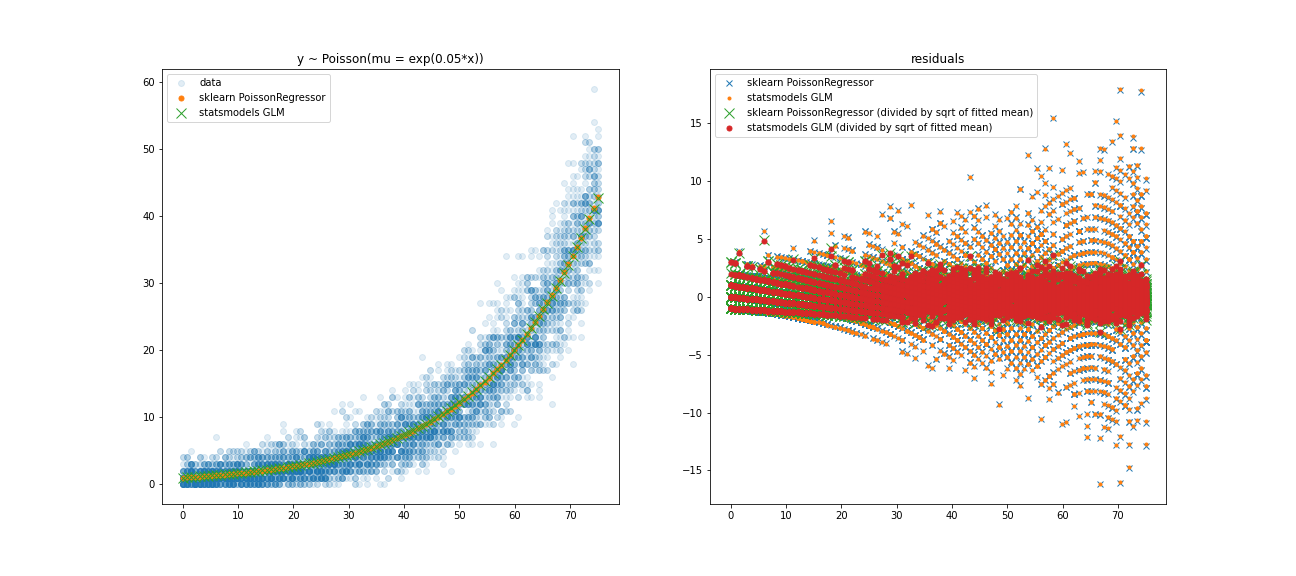
\includegraphics[width=\textwidth]{poissonmodels02.png}
    \caption{Left: Ordinary Poisson Regression on data that satisfies the assumptions of the model. For small rates, the model is approximately linear, but beyond that it shows exponential growth because of the log-link. Right: Residuals showing heteroskedasticity with variance increasing with the mean. Dividing the residuals by the mean yields constant variance.}
    \label{fig:ordinarypoisson}
\end{figure}


\subsubsection{Poisson Noise \& Central Limit Theorem}

For small count rates, the Poisson distribution is highly skewed and strictly positive. For large count rates, the Poisson distribution is essentially normal, except that variance and mean are locked.

If you are dealing with large counts, then the Poisson model still has the feature of being heteroskedastic.

\subparagraph{Advantages of using Poisson Noise}

\begin{itemize}
\item The Poisson Distribution is highly skewed for small rates, and strictly positive. For high enough count rates, this advantage disappears.
\item The Poisson Distribution is heteroskedastic
\end{itemize}

\subparagraph{Drawbacks of using Poisson Noise}

\begin{itemize}
\item The Poisson distribution only has a single parameter. The assumption that the mean and the variance are the same is very restrictive.
\end{itemize}


\begin{figure}
\centering
    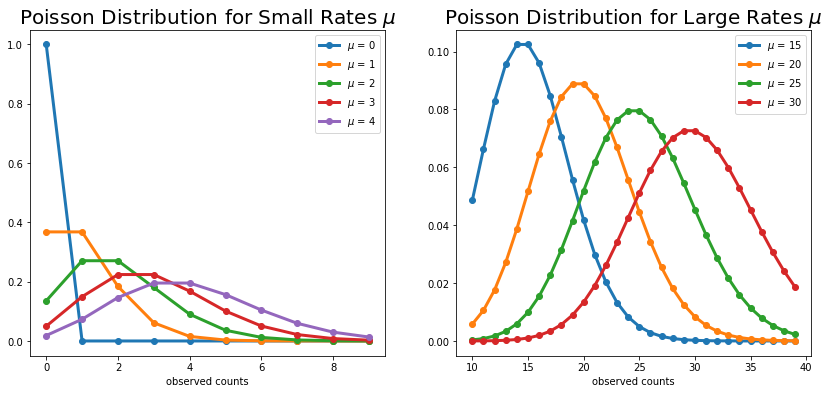
\includegraphics[width=\textwidth]{poissonmodels01.png}
    \caption{Left: The Poisson Distribution for small rates is highly skewed. Right: The Poisson Distribution for intermediate rates looks very similar to a normal distribution. In both cases, the variance and the mean are the same value.}
    \label{fig:poissonandcentrallimit}
\end{figure}


\subsubsection{Poisson Noise Analogy to Least Squares Regression}
To anchor intuition in familiar territory, consider least squares regression with a log-linear relationship between endogenous and exogenous variables (that is, the model assumes a relationship of $log(y)=a + \mathbf{bx}$ that is beset with Gaussian noise). The familiar form for the model is:

\begin{equation}
\begin{array}{rl}
y &= a\exp{\mathbf{b \cdot x}} + \epsilon \\
&= \exp\mathbf{\beta \cdot x} + \epsilon
\end{array}
\end{equation}

Where the constant $a$ was absorbed into the coefficient vector $\mathbf{\beta}$ in the second line, and $\mathbf{x} \rightarrow [1,\mathbf{x}]$. $\epsilon$ is an error term that is assumed to have normal distribution with zero mean, i.e. $\epsilon \sim \mathscr{N}(0,\sigma)$. It's a bit unnatural, but this can be rewritten, absorbing the parameters into the random term:

\begin{equation}
y = 0 + \epsilon'
\end{equation}

With $\epsilon' \sim \mathscr{N}(\mu = \exp{\mathbf{\beta \cdot x}},\sigma)$. Now what if the fluctuations aren't normally distributed about the mean, but they are Poisson distributed about the mean? In that case, $\epsilon' \sim \mathrm{Poisson}(\mu = \exp{\mathbf{\beta \cdot x}})$. 



\subsubsection{Multivariate Poisson Model}
For least squared regression, it's totally common to look at multivariate models with interesting codependence structure captured by a covariance matrix. In analogy to that, there is multivariate Poisson Regression. The math looks quite different. 

\url{http://www2.stat-athens.aueb.gr/~karlis/multivariate%20Poisson%20models.pdf}

\subsubsection{Goodness of Fit}
The Poisson deviance is given by:

\begin{equation}
D = 2\sum\left\{ y_i \log\left( \frac{y_i}{\hat{\mu}_i} \right) - \left( y_i - \hat{\mu}_i \right) \right\}
\end{equation}

Here, $\hat{\mu}_i = e^{\mathbf{x}^T_i \hat{\mathbf{\beta}}}$ is the fitted mean of the $i$th data point, and $y_i$ is the observed count of the $i$th datapoint. 

For large sample sizes, the deviance will be distributed approximately chi-squared with $n-p$ degrees of freedom, where $n$ is the number of data points and $p$ is the number of features. An alternative to the deviance is Pearson's chi-squared statistic. 

\subsubsection{General $\mu = f(\mathbf{x})$}
The Poisson-ness only has to do with how the data fluctuates about the mean. How the mean is expected to depend on the explanatory variables is another question. In so far, general other functions, including highly-nonlinear machine learning models, can be fit under the assumption of Poisson noise.

XGBoost supports poisson loss. Empirically, it seems that Poisson loss performs worse in the regime where the model is underfitting, and slightly better in the regime where the model is overfitting. The difference is especially pronounced in the Poisson deviance and for sparse data.


\begin{figure}
\centering
    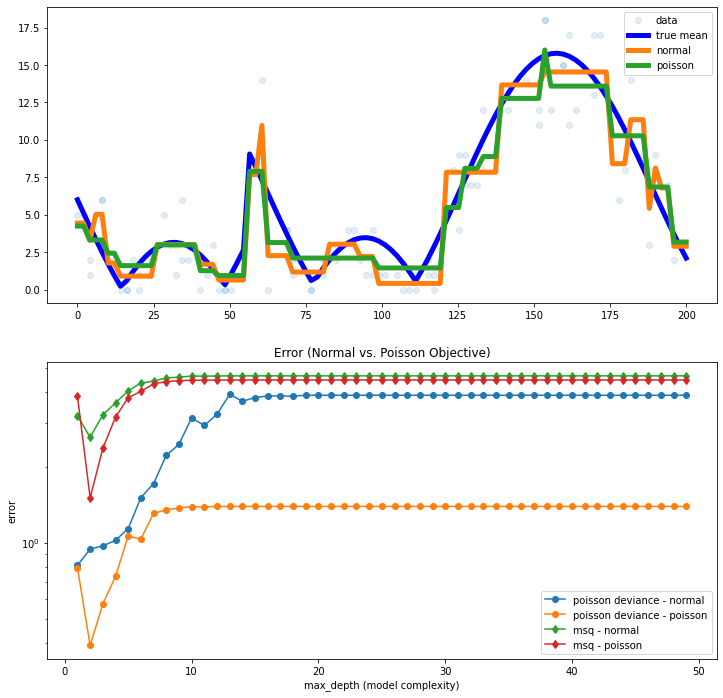
\includegraphics[width=\textwidth]{poissonmodels03.png}
    \caption{Left: Ordinary Poisson Regression on data that satisfies the assumptions of the model. For small rates, the model is approximately linear, but beyond that it shows exponential growth because of the log-link. Right: Residuals showing heteroskedasticity with variance increasing with the mean. Dividing the residuals by the mean yields constant variance.}
    \label{fig:ordinarypoisson}
\end{figure}